\section{Lezione del 16/01/19 [Tantari]}
\textcolor{red}{Introduzione e road map vanno riviste quando avrò finito la seconda lezione e sarà chiaro (spero) cosa si sta cercando di fare.}

Ci prefiggiamo di studiare ora il modello di Curie-Weiss nel \emph{limite termodinamico}, cioè nel limite in cui il numero $ n $ di particelle tende a infinito. In particolare calcoleremo il limite dell'energia libera $ f_{\beta, n} \coloneqq F_{\beta, n}/n = -\frac{\log Z_{\beta, n}}{\beta n}$\footnote{D'ora in poi ometteremo il pedice $ \beta $ per alleggerire la notazione.}.

\subsubsection{Road map}
\begin{enumerate}
  \item Calcolo di $ \lim_{n\to\infty} \frac{1}{n} \log{Z_n} = \lim_{n\to\infty} -\frac{\beta F_n}{n} $
  \item Data una generica osservabile $ \mathcal{O}\colon\Sigma\to\R $, calcoliamone il valore atteso nel limite termodinamico $ \lim_{n\to\infty} \mean{\mathcal{O}_n(\sigma)}_{P_\beta} $. Nel nostro caso considereremo la \emph{magnetizzazione media} $ m_n(\sigma) \coloneqq \mean{\frac{1}{n}\sum_{i=1}^{n}\sigma_i}_{P_\beta} $.
  \item \textcolor{red}{Automedia: calcolo delle fluttuazioni delle osservabili}.
  $ \lim_{n\to\infty} P_\beta\left(\ \abs{m_n(\sigma) - m_\beta } > \epsilon \right) $.
  \textcolor{red}{Non capisco cosa sia $ m_\beta $ e se quella che prima ho definito come $ m_n $ sia davvero $ m_n $ oppure sia $ m_\beta $.}
\end{enumerate}

Nel modello di Curie-Weiss lo spazio delle fasi è $ \Sigma = \{-1,1\}^n $. L'hamiltoniana è:
\[ \ham_n(\sigma) = -\frac{1}{n} \sum_{i<j} \sigma_i \sigma_j - h \sum_i \sigma_i \]
dove il primo termine descrive l'interazione tra gli spin, che tendono ad allinearsi, e il secondo l'interazione con il campo esterno $ h $. Osserviamo che $ \ham_n $ scala come $ n $; una quantità di questo tipo di dice \emph{intensiva}. La quantità che ci prefiggiamo di calcolare, $ f_n $, è invece \emph{intensiva}.

Cominciamo riscrivendo l'hamiltoniana in termini di $ m_n(\sigma) $:
\[ \sum_{i<j} \sigma_i \sigma_j = \frac{1}{2} \sum_{i \neq j} \sigma_i \sigma_j = \sum_{i,j} \sigma_i \sigma_j -\frac{n}{2} = \frac{n^2 m_n^2(\sigma)}{2} - \frac{n}{2} \]
da cui, trascurando un'irrilevante costante additiva
\[ \ham(\sigma) = -\frac{n m_n^2(\sigma)}{2} - hnm_n(\sigma) \]
e quindi
\[ Z_n = \sum_{\sigma \in \Sigma} \exp\left( \frac{\beta n m_n^2(\sigma)}{2} + \beta h n m_n(\sigma) \right) \]

\subsection{Esistenza del limite}
Dimostriamo innanzi tutto che il limite $ \lim_{n\to\infty} \frac{\log Z_n}{n} $ esiste.
\begin{proof}
    Procediamo facendo vedere che la successione $ \log Z_n $ è subadditiva e usiamo il lemma \ref{lem:fekete}.
    Posto $ n = n_1 + n_2 $, siano $ \sigma_1 \in \{-1,1\}^{n_1} $ e $ \sigma_2 \in \{-1,1\}^{n_2} $; si ha
    \[ m_n(\sigma_1,\sigma_2) = \frac{n_1}{n} m_1(\sigma_1) + \frac{n_2}{n} m_2(\sigma_2) \]
    si verifica con facili calcoli che
    \[ n m_n^2 = n_1 m_1^2 + n_2 m_2^2 - \frac{n_1 n_2}{n} (m_1-m_2)^2 \leq n_1 m_1^2 + n_2 m_2^2 \]
    e quindi
    \begin{align*}
        Z_{n_1} Z_{n_2} & = \sum_{\sigma_1\in\Sigma_1} \sum_{\sigma_2\in\Sigma_2} \exp\left(\frac{\beta}{2} \left(n_1 m_{n_1}^2(\sigma_1) + n_2 m_{n_2}^2(\sigma_2) \right) \right) \exp\left(\beta h\left(n_1 m_{n_1}(\sigma_1) + n_2 m_{n_2}(\sigma_2) \right) \right) \\
                        & \geq \sum_{\sigma\in\Sigma} \exp\left(\frac{\beta n m_n^2(\sigma)}{2} \right) \exp\left(\beta h n m_n(\sigma) \right) = Z_{n_1+n_2}.
    \end{align*}
    Prendendo il logaritmo si ottiene $ \log Z_{n_1+n_2} \leq \log Z_{n_1} + \log Z_{n_2} $.
\end{proof}

Possiamo ora dare una stima grossolana del limite in analisi. \textcolor{red}{(Non ne ho capito il senso)}. In un verso abbiamo:
\[ Z_n = \sum_{\sigma \in \Sigma} \exp\left( \frac{\beta n m_n^2(\sigma)}{2} + \beta h n m_n(\sigma) \right) \leq \sum_{\sigma \in \Sigma} \exp\left(  \frac{\beta n}{2} + \beta n h \right) = \exp\left( n \left( \log 2 + \frac{\beta}{2} + \beta h \right) \right) \]
Da cui
\[ \frac{\log Z_n}{n} \leq \log 2 + \frac{\beta}{2} + \beta h \]
Nell'altro verso, detta $ U $ la distribuzione uniforme sulle $ 2^n $ configurazioni possibili, e usando la diseguaglianza di Jensen, si ha
\[ Z_n = 2^n \mean{\exp\left(-\beta\ham_n\right)}_U \geq 2^n \exp\left( -\beta \mean{\ham}_U \right) = 2^n \]
in quanto $ \mean{\sigma_i}_U = 0 $ e $ \mean{\sigma_i\sigma_j}_U = \mean{\sigma_i}_U\mean{\sigma_j}_U = 0 $. Prendendo il logaritmo abbiamo infine:
\[ \frac{\log Z_n}{n} \geq \log 2 \]
\textcolor{red}{Abbiamo usato il principio variazionale di Gibbs???}

\subsection{Calcolo dell'energia libera}
Calcoliamo ora in modo esatto l'energia libera nel limite termodinamico.
\subsubsection{Primo bound}
Sia $ M \in [-1,1] $. Allora si ha $ \exp\left( -\frac{\beta n (m_n(\sigma) - M)^2}{2} \right) \leq 1 $ e quindi
\begin{align*}
    Z_n & \geq \sum_{\sigma \in \Sigma} \exp\left( \frac{\beta n m_n^2(\sigma)}{2} + \beta h n m_n(\sigma) - \frac{\beta n (m_n(\sigma)-M)^2}{2}\right) \\
        & = \exp\left( -\frac{\beta n M^2}{2} \right) \sum_{\sigma \in \Sigma} \exp\left( (M+h) \beta n m_n(\sigma) \right)                              \\
        & = \exp\left( -\frac{\beta n M^2}{2} \right) \sum_{\sigma \in \Sigma} \prod_{i=1}^{n} \exp( \beta(M+h) \sigma_i )                               \\
        & = \exp\left( -\frac{\beta n M^2}{2} \right) \sum_{\sigma_1 = \pm 1} \cdots \sum_{\sigma_n = \pm 1} \prod_{i=1}^{n} \exp( \beta(M+h) \sigma_i ) \\
        & = \exp\left( -\frac{\beta n M^2}{2} \right) \left(\sum_{\sigma_1 = \pm 1} \exp(\beta(M+h)\sigma_1)\right) \cdots \left(\sum_{\sigma_n = \pm 1} \exp(\beta(M+h)\sigma_n)\right) \\
        & = \exp\left( -\frac{\beta n M^2}{2} \right) \prod_{i=1}^{n} \sum_{\sigma_i = \pm 1} \exp(\beta(M+h)\sigma_i) \\
        & = \exp\left( -\frac{\beta n M^2}{2} \right) 2^n \cosh^n(\beta(M+h)). \\
\end{align*}
Abbiamo dunque:
\[ \frac{\log Z_n}{n} \geq \log 2 + \log\cosh(\beta(M+h)) - \frac{\beta M^2}{2} \eqqcolon \alpha(\beta, h) \]
Prendendo il limite per $ n\to\infty $ e il $ \sup $ al variare di $ M $ in $ [-1,1] $ otteniamo
\[ \lim_{n \to +\infty}\frac{\log Z_n}{n} \geq \sup_{M\in[-1,1]} \alpha(M, \beta, h) \eqqcolon \bar{\alpha}(\beta, h) \]

\subsubsection{Secondo bound}
Osserviamo che $ m_n(\sigma) $ può assumere solamente $ n+1 $ valori: $ \im m_n = \left\{ -1, -1 + \frac{2}{n}, \ldots, 1-\frac{2}{n}, 1 \right\} $. Sia ora $ M \in \im m_n $; abbiamo che
\[ \sum_{M\in \im m_n} \exp\left( -\frac{\beta(m(\sigma)-M)^2}{2} \right) = 1 + \sum_{\substack{M \in \im m_n \\ M \neq m_n(\sigma)}} \exp\left( -\frac{\beta(m(\sigma)-M)^2}{2} \right) \geq 1 \]
e quindi
\begin{align*}
    Z_n & \leq \sum_{M\in \im m_n} \sum_{\sigma \in \Sigma} \exp\left( \frac{\beta n m_n^2(\sigma)}{2} + \beta h n m_n(\sigma) - \frac{\beta n (m_n(\sigma)-M)^2}{2}\right)     \\
        & = \sum_{M\in \im m_n} \exp\left( n \alpha(M, \beta, h) \right)
         \leq \sum_{M\in \im m_n} \exp(n \bar{\alpha}(\beta, h)) = (n+1) \exp(n \bar{\alpha}(\beta, h)).
\end{align*}
Prendendo il logaritmo e facendo il limite si ottiene
\[  \lim_{n \to +\infty} \frac{\log Z_n}{n} \leq \bar{\alpha}(\beta,h). \]
Dunque abbiamo dimostrato che
\[ \lim_{n \to +\infty}\frac{\log Z_n}{n} = \bar{\alpha}(\beta,h) = \sup_{M\in[-1,1]} \alpha(M, \beta, h). \]

Studiamo ora i punti stazionari di $ \alpha(M, \beta, h) $ a fissati $ \beta $ e $ h $:
\begin{equation}\label{eq:mbar}
    \pd{\alpha}{M} = \beta \left( \tanh(\beta (M+h)) - M \right) = 0.
\end{equation}
Nel caso particolare $ h = 0 $, cioè in assenza di campo esterno, l'equazione si riduce a $ \tanh{\beta M} = M $. Questa ha sempre la soluzione $ M = 0 $, mentre solo nel caso $ \beta > 1 $ si aggiungono due soluzioni opposte non nulle. Inoltre in un intorno destro di $ M = 0 $ la derivata $ \pd{\alpha}{M} $ è negativa per $ \beta \leq 1 $, positiva per $ \beta > 1 $. Dunque in $ M = 0 $ $ \alpha $ presenta un massimo per $ \beta \leq 1 $, mentre un minimo per $ \beta > 1 $. Si verifica infine che le soluzioni aggiuntive presenti nel caso $ \beta > 1 $ corrispondono a due massimi (si veda anche la figura \ref{fig:alpha}).

Nel seguito porremo $ \bar{M}(\beta,h) \coloneqq \argmax_{M\in[-1,1]} \alpha(M,\beta,h) $ e dunque sarà $ \bar{\alpha}(\beta, h) = \alpha(\bar{M}, \beta, h) $\footnote{In caso di ambiguità si scelga, ad esempio, il più grande $ M $ che realizzano il massimo.}. Nella figura \ref{fig:transizione} è riportato l'andamento di $ \pm \bar{M}(\beta, 0) $ in funzione di $ T=\frac{1}{\beta} $. Si osserva che in corrispondenza di $ \beta = 1 $ il sistema presenza una transizione di fase \textcolor{red}{di seconda specie}.

\iffigureon
\begin{figure}[p]
    \centering
    \subfloat{%<<<<<<<WARNING>>>>>>>
% PGF/Tikz doesn't support the following mathematical functions:
% cosh, acosh, sinh, asinh, tanh, atanh,
% x^r with r not integer

% Plotting will be done using GNUPLOT
% GNUPLOT must be installed and you must allow Latex to call external
% programs by adding the following option to your compiler
% shell-escape    OR    enable-write18 
% Example: pdflatex --shell-escape file.tex 

\definecolor{sexdts}{rgb}{0.1803921568627451,0.49019607843137253,0.19607843137254902}
\begin{tikzpicture}[line cap=round,line join=round,>=triangle 45,x=1cm,y=1cm]
\begin{axis}[
x=1cm,y=1cm,
axis lines=middle,
xmin=-3.5,
xmax=3.5,
ymin=-1.7498317317715488,
ymax=2.781986295604104,
xtick={-4,-3.5,...,3},
ytick={-1.5,-1,...,2.5},
xticklabels={,,},
yticklabels={,,},
xlabel=$M$,
ylabel={$\alpha(M,\beta>1,0)$},]
\clip(-4.053984304681382,-1.7498317317715488) rectangle (4.4441428338333075,2.781986295604104);
\draw[line width=1pt,color=sexdts,smooth,samples=100,domain=-4.053984304681382:4.4441428338333075] plot(\x,{ln(2)+ln(cosh(2.2*((\x))))-1/2*2.2*(\x)^(2)});
\end{axis}
\end{tikzpicture}}
    \subfloat{%<<<<<<<WARNING>>>>>>>
% PGF/Tikz doesn't support the following mathematical functions:
% cosh, acosh, sinh, asinh, tanh, atanh,
% x^r with r not integer

% Plotting will be done using GNUPLOT
% GNUPLOT must be installed and you must allow Latex to call external
% programs by adding the following option to your compiler
% shell-escape    OR    enable-write18 
% Example: pdflatex --shell-escape file.tex 

\definecolor{sexdts}{rgb}{0.1803921568627451,0.49019607843137253,0.19607843137254902}
\begin{tikzpicture}[line cap=round,line join=round,>=triangle 45,x=1cm,y=1cm]
\begin{axis}[
x=1cm,y=1cm,
axis lines=middle,
xmin=-3.5,
xmax=3.5,
ymin=-1.7498317317715488,
ymax=2.781986295604104,
xtick={-4,-3.5,...,3},
ytick={-1.5,-1,...,2.5},
xticklabels={,,},
yticklabels={,,},
xlabel=$M$,
ylabel={$\alpha(M,\beta\leq 1,0)$},]
\clip(-4.053984304681382,-1.7498317317715488) rectangle (4.4441428338333075,2.781986295604104);
\draw[line width=1pt,color=sexdts,smooth,samples=100,domain=-4.053984304681382:4.4441428338333075] plot(\x,{ln(2)+ln(cosh(0.7*((\x))))-1/2*0.7*(\x)^(2)});
\end{axis}
\end{tikzpicture}} \\
    \subfloat{%<<<<<<<WARNING>>>>>>>
% PGF/Tikz doesn't support the following mathematical functions:
% cosh, acosh, sinh, asinh, tanh, atanh,
% x^r with r not integer

% Plotting will be done using GNUPLOT
% GNUPLOT must be installed and you must allow Latex to call external
% programs by adding the following option to your compiler
% shell-escape    OR    enable-write18 
% Example: pdflatex --shell-escape file.tex 

\definecolor{sexdts}{rgb}{0.1803921568627451,0.49019607843137253,0.19607843137254902}
\begin{tikzpicture}[line cap=round,line join=round,>=triangle 45,x=1cm,y=1cm]
\begin{axis}[
x=1cm,y=1cm,
axis lines=middle,
xmin=-3.5,
xmax=3.5,
ymin=-1.7498317317715488,
ymax=2.781986295604104,
xtick={-4,-3.5,...,3},
ytick={-1.5,-1,...,2.5},
xticklabels={,,},
yticklabels={,,},
xlabel=$M$,
ylabel={$\alpha(M,\beta>1,h>0)$},]
\clip(-4.053984304681382,-1.7498317317715488) rectangle (4.4441428338333075,2.781986295604104);
\draw[line width=1pt,color=sexdts,smooth,samples=100,domain=-4.053984304681382:4.4441428338333075] plot(\x,{ln(2)+ln(cosh(2.3*((\x)+0.2)))-1/2*2.3*(\x)^(2)});
\end{axis}
\end{tikzpicture}}
    \subfloat{%<<<<<<<WARNING>>>>>>>
% PGF/Tikz doesn't support the following mathematical functions:
% cosh, acosh, sinh, asinh, tanh, atanh,
% x^r with r not integer

% Plotting will be done using GNUPLOT
% GNUPLOT must be installed and you must allow Latex to call external
% programs by adding the following option to your compiler
% shell-escape    OR    enable-write18 
% Example: pdflatex --shell-escape file.tex 

\definecolor{sexdts}{rgb}{0.1803921568627451,0.49019607843137253,0.19607843137254902}
\begin{tikzpicture}[line cap=round,line join=round,>=triangle 45,x=1cm,y=1cm]
\begin{axis}[
x=1cm,y=1cm,
axis lines=middle,
xmin=-3.5,
xmax=3.5,
ymin=-1.7498317317715488,
ymax=2.781986295604104,
xtick={-4,-3.5,...,3},
ytick={-1.5,-1,...,2.5},
xticklabels={,,},
yticklabels={,,},
xlabel=$M$,
ylabel={$\alpha(M,\beta>1,h<0\textsl{})$},]
\clip(-4.053984304681382,-1.7498317317715488) rectangle (4.4441428338333075,2.781986295604104);
\draw[line width=1pt,color=sexdts,smooth,samples=100,domain=-4.053984304681382:4.4441428338333075] plot(\x,{ln(2)+ln(cosh(2.3*((\x)-0.2)))-1/2*2.3*(\x)^(2)});
\end{axis}
\end{tikzpicture}}
    \caption{$ \alpha(M,\beta,h) $ per diversi valori di $ \beta $ e $ h $ fissati.}
    \label{fig:alpha}
\end{figure}
\begin{figure}[p]
    \centering
    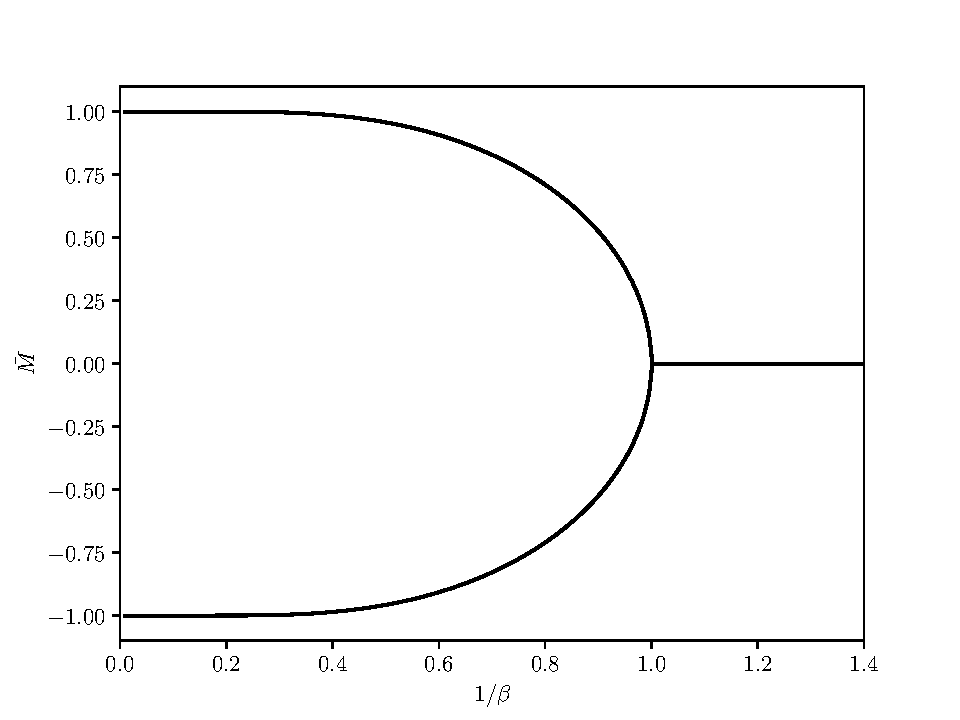
\includegraphics[scale=0.8]{img/cw/transizione.pdf}
    \caption{$ \bar{M} $ in funzione di $ T = \frac{1}{\beta}$.}
    \label{fig:transizione}
\end{figure}
\fi

\subsubsection{Valore atteso della magnetizzazione media}
Sfruttiamo ora la conoscenza del limite termodinamico dell'energia libera per calcolare il valore atteso della magnetizzazione media e del suo quadrato. Dimostriamo innanzi tutto la seguente
\begin{proposition}
    Siano $ f_n\colon I\subseteq\R \to \R $ funzioni convesse e derivabili in $ x_0 \in I $ e sia $ f\colon I\to\R $ derivabile in $ x_0 $ tale che $ f_n \to f $ puntualmente. Allora
    \[ \lim_{n \to +\infty} f_n'(x_0) = f'(x_0) = \od{}{x} \left( \lim_{n \to +\infty} f'(x_0) \right). \]
\end{proposition}
\begin{proof}\label{prop:convessascambio}
    Sia $ \Delta x \geq 0 $.
    \[ f_n'(x_0) \leq \frac{f_n(x_0+\Delta x)-f_n(x_0)}{\Delta x}. \]
    Prendendo il $ \limsup $ si ha
    \[ \limsup_{n\to +\infty} f'_n(x_0) \leq \frac{f(x_0+\Delta x)-f(x_0)}{\Delta x} \]
    che nel limite $ \Delta x \to 0 $ diventa
    \[ \limsup_{n\to +\infty} f'_n(x_0) \leq f'(x_0). \]
    Analogamente si mostra che vale
    \[ \liminf_{n\to +\infty} f_n'(x_0) \geq f'(x_0) \]
    da cui la tesi.
\end{proof}

Calcoliamo ora
\[ \pd{}{h}\left(\frac{\log Z_n}{n}\right) = \frac{1}{n Z_n} \pd{Z_n}{h} = \frac{1}{nZ_n}\sum_{\sigma \in \Sigma} \exp\left( \frac{\beta n m_n^2(\sigma)}{2} + \beta h n m_n(\sigma) \right) \beta n m_n(\sigma) = \beta \mean{m_n}_{P_\beta}. \]
Abbiamo quindi
\begin{align}
	\label{eq:limmagnmedia}
    \lim_{n \to +\infty}\mean{m_n}_{P_\beta} & = \frac{1}{\beta} \lim_{n \to +\infty} \dpd{}{h}\left(\frac{\log Z_n}{n}\right) = \frac{1}{\beta} \dpd{}{h} \left( \lim_{n \to +\infty} \frac{\log Z_n}{n} \right) \nonumber \\
	                                         & = \frac{1}{\beta} \dpd{\bar{\alpha}}{h}(\beta, h) = \frac{1}{\beta} \dod{}{h} \left( \alpha(\bar{M}(\beta,h), \beta, h)\right) \nonumber \\
                                             & = \frac{1}{\beta} \left[ \dpd{\alpha}{M}(\bar{M}(\beta,h),\beta,h) \dpd{\bar{M}}{h}(\beta,h) + \dpd{\alpha}{h}(\bar{M}(\beta,h),\beta,h) \right] \nonumber \\
                                             & = \tanh(\beta(\bar{M}(\beta,h)+h))  \nonumber \\
                                             & = \bar{M}(\beta, h)
\end{align}
dove si è sostituita la condizione \eqref{eq:mbar} e si sono scambiati limite e derivata per la proposizione \ref{prop:convessascambio}. Se invece deriviamo rispetto a $ \beta $ otteniamo
\begin{align*}
    \dpd{}{\beta} \left(\frac{\log Z_n}{n}\right) &= \frac{1}{n Z_n} \dpd{Z_n}{\beta} = \frac{1}{n Z_n} \sum_{\sigma \in \Sigma} \exp\left( \frac{\beta n m_n^2(\sigma)}{2} + \beta h n m_n(\sigma) \right) \left( \frac{n m_n^2(\sigma)}{2} + hnm_n(\sigma) \right) \\ &= \frac{1}{2} \mean{m_n^2}_{P_\beta} + h \mean{m_n}_{P_\beta}
\end{align*}
da cui
\begin{align*}
	\frac{1}{2}\lim_{n \to +\infty}\mean{m_n^2}_{P_\beta} + h\lim_{n \to +\infty}\mean{m_n}_{P_\beta}& = \lim_{n \to +\infty} \dpd{}{\beta} \left(\frac{\log Z_n}{n}\right) = \dpd{}{\beta} \left( \lim_{n \to +\infty}\frac{\log Z_n}{n} \right) \\
                                               & = \dpd{\bar{\alpha}}{\beta}(\beta,h) = \dod{}{\beta}\left(\alpha(\bar{M}(\beta,h),\beta,h)\right) \\
                                               & = \dpd{\alpha}{M}(\bar{M}(\beta,h),\beta,h) \dpd{\bar{M}}{\beta}(\beta,h) + \dpd{\alpha}{\beta}(\bar{M}(\beta,h),\beta,h) \\
                                               & = \left(\bar{M}(\beta,h) + h\right) \tanh\left(\beta(\bar{M}(\beta,h)+ h)\right) - \frac{1}{2}\bar{M}^2(\beta,h)\\
                                               & = \frac{1}{2}\bar{M}^2(\beta,h) + h \bar{M}(\beta,h).
\end{align*}
Usando la \ref{eq:limmagnmedia} segue che
\[ \lim_{n \to +\infty} \mean{m_n^2}_{P_\beta} = \bar{M}^2(\beta,h). \]
\textcolor{red}{Qui mancano un po' di discorsi conclusivi che però vengono ripresi nella lezione successiva.}

